
%
%  $Description: Author guidelines and sample document in LaTeX 2.09$ 
%
%  $Author: ienne $
%  $Date: 1995/09/15 15:20:59 $
%  $Revision: 1.4 $
%

\documentclass[times, 10pt,twocolumn]{article} 
\usepackage{paper}
\usepackage{times}
\usepackage{graphicx}
\usepackage{float}

%\documentstyle[times,art10,twocolumn,latex8]{article}

%------------------------------------------------------------------------- 
% take the % away on next line to produce the final camera-ready version 
\pagestyle{empty}

%------------------------------------------------------------------------- 
\begin{document}

\title{Citi Bike Usage Balancing through Congestion Pricing}

\author{Paul Griffioen\\Dept. of Electrical and Computer Engineering\\Carnegie Mellon University\\ pgriffi1@andrew.cmu.edu\\
% For a paper whose authors are all at the same institution, 
% omit the following lines up until the closing ``}''.
% Additional authors and addresses can be added with ``\and'', 
% just like the second author.
\and
Anthony Jin\\Dept. of Electrical and Computer Engineering\\Carnegie Mellon University\\xiaoxiaj@andrew.cmu.edu\\
}

\maketitle
\thispagestyle{empty}

%------------------------------------------------------------------------- 
\Section{Abstract}

The issue of congestion in bicycle sharing systems is prevalent in many cities. This project proposes an incentive-based pricing scheme for the Citi Bike system that minimizes bicycle congestion. It approaches bicycle sharing systems from a network perspective, analyzing and optimizing the network by providing monetary incentives to users.

%------------------------------------------------------------------------- 
\Section{Introduction and Motivation}

The Citi Bike system, located in New York City, is one of many bicycle sharing systems that exist in the world. Since users unlock a bike at one station and drop it off at another station, bikes tend to follow unidirectional flows at various times of the day. As a result, some stations have few to no bikes at them while others are completely full.

This unidirectional flow of bikes frustrates users who would like to pick up a bike from an empty station or drop off a bike at a full station. As a result, this project seeks to address the issue of system congestion through a pricing scheme based on the optimization of network structure and dynamics. In addition, alteration of the network topology to reduce congestion will be explored through optimal placement of nodes (stations). In the end, this project seeks to analyze the Citi Bike network and to minimize congestion by modifying its structure through changing people's incentives.

%------------------------------------------------------------------------- 
\Section{Previous Work}

Previous work has taken many viewpoints to solve the bike sharing congestion problem. The work in \cite{incentives} proposes a dynamic incentives system that involves future traffic prediction, truck-based re-positioning policies, and schema to compute monetary incentives for users. The authors in \cite{redistribution} use a similar approach, combining staff-based dynamic vehicle distribution and real-time pricing incentives for customers. In contrast, \cite{management} and \cite{redistribution} look at the inventory management of individual bike-sharing stations and formulate appropriate convex optimization problems. Similar to the aforementioned approaches, this project will address the congestion problem as a convex optimization problem and introduce a congestion-based pricing scheme to modify user incentives. Unlike prior work, however, it takes a network standpoint and models the Citi Bike system as a dynamic network.

%------------------------------------------------------------------------- 
\Section{Approach}

The Citi Bike network is built using available data from Citi Bike's website \cite{dataset}. The nodes represent different bike stations and the weighted links represent the number of trips made from one station to another in a certain period of time. In addition, each node contains information such as the station's identification number, latitude and longitude, maximum capacity, and the current number of bikes at the station. These node attributes will be used as the inputs in the convex optimization problem for the incentive-based pricing scheme.

The trip data in \cite{dataset} does not include explicit information about the addition or removal of bikes to the system or the transfer of bikes by truck from one station to another. Consequently, this project can only analyze bike trips from one station to another. In addition, there is no information about the number of bikes at particular stations at specific points in time. As a result, an initialization procedure is used to infer this information. A start time is identified, and it is assumed that no bikes are in the system at this start time. Over a specified time period, bikes are added to the system using incoming trip data for each station. Bikes are then tracked by identification number to determine which station they are at. At the end of this period, it is assumed that all bikes have been added to the system and each station is assigned with an initial number of bikes. Future trip data can now be used to determine the number of bikes at particular stations at any time after the initialization procedure.

%------------------------------------------------------------------------- 
\Section{Experimental Setup and Practical Results}
Using the approach described in the previous section, a sample dynamic network is constructed to represent bike usage from Thursday to Saturday in a normal week. First, Citi Bike data from the first three days of September 2016 is extracted from the original data set in \cite{dataset} to generate a node table with 583 nodes and an edge list with more than 130,000 edges. Second, the node table and edge list are imported to Gephi as a dynamic network. The Gephi plugin \textit{Geo Layout} is used to arrange the nodes according to their geographic locations, while network properties are dynamically changed by filtering out edges outside a particular time window. In this analysis, the time window for edge filtering is set to one hour.\\

%\begin{figure}[H]
%	\centering
%	\includegraphics[width=0.5\textwidth]{combined.jpg}
%	\caption{Citi Bike network at four time intervals on September 1, 2016}
%\end{figure}
\centerline{\includegraphics[width=0.5\textwidth]{m2/combined.jpg}}
\centerline{Figure 1: Citi Bike Network on September 1, 2016}

Figure 1 shows the network at four different time intervals on September 1, 2016. From left to right, the figures represent the network between 1\textsc{am} and 2\textsc{am}, 7\textsc{am} and 8\textsc{am}, 1\textsc{pm} and 2\textsc{pm}, and 7\textsc{pm} and 8\textsc{pm}. Figure 2 illustrates how some of the network properties change over time. Every day, the maximum average node degree is observed between 4\textsc{pm} and 7\textsc{pm}, corresponding to the evening rush hour. On the two weekdays, there is also a secondary peak between 7\textsc{am} and 8\textsc{am}, reflecting the morning rush hour. As expected, this secondary peak is not present on September 3 since it is a Saturday. On the contrary, the network's average path length stays relatively consistent during the day and in the early evening. Bikers seem to take longer trips around midnight and in the morning (between 6\textsc{am} and 7\textsc{am}), while the trips between midnight and 6\textsc{am} tend to be much shorter. As for community structure, the network's modularity and formation of communities exhibit a periodic pattern; during the day, the network has high modularity and the nodes can be grouped into a few communities. At night, the network is less modular and only a handful of nodes can form communities with others.

This experimental setup has some limitations. For example, the congestion level at each station (i.e. maximum capacity versus current number of stored bikes) is not taken into account because the initialization procedure has not been implemented. In addition, the distance between each pair of nodes is assumed to be the same while a more realistic analysis should also take into account the physical distance between stations. Lastly, this analysis has only exploited a very small subset of the available data.

%% Insert figs
%\begin{figure}[H]
%	\centering
%	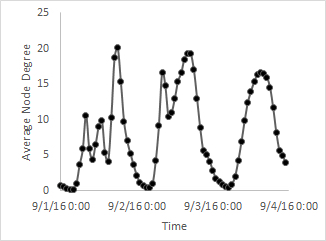
\includegraphics[width=0.5\textwidth]{node_degree.jpg}
%	\caption{Average node degree}
%\end{figure}

%\centerline{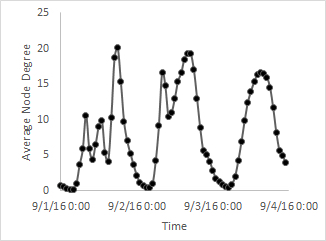
\includegraphics[width=0.4\textwidth]{node_degree.jpg}}
%\centerline{Figure 2: Average Node Degree}
%\vspace{5mm}

%\begin{figure}[H]
%	\centering
%	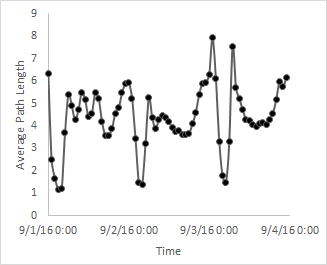
\includegraphics[width=0.5\textwidth]{path_length.jpg}
%	\caption{Average path length}
%\end{figure}

%\centerline{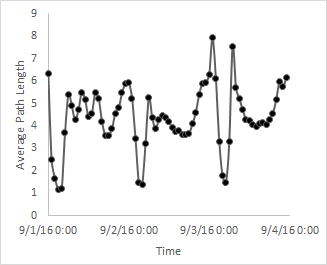
\includegraphics[width=0.4\textwidth]{path_length.jpg}}
%\centerline{Figure 3: Average Path Length}
%\vspace{5mm}

%\begin{figure}[H]
%	\centering
%	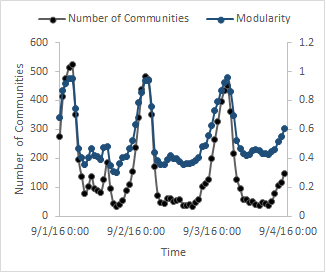
\includegraphics[width=0.5\textwidth]{communities.jpg}
%	\caption{Modularity and number of communities}
%\end{figure}

%\centerline{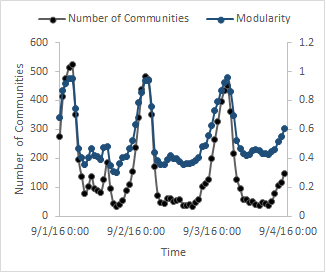
\includegraphics[width=0.4\textwidth]{communities.jpg}}
%\centerline{Figure 4: Modularity and Number of Communities}

\centerline{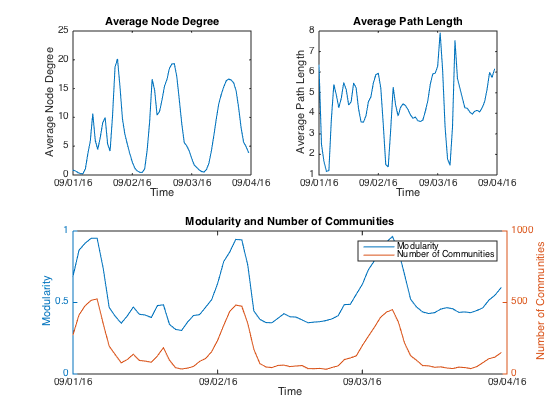
\includegraphics[width=0.5\textwidth]{m2/plotterfigure.png}}
\centerline{Figure 2: Citi Bike Network Properties}

%------------------------------------------------------------------------- 
\Section{Conclusion and Short-Term Plans}
The basic methodology to construct the Citi Bike network is proposed in this work. Because certain information is not available about the bike stations' capacity, an initialization procedure is also proposed to estimate the number of bikes in the system and at each station. As a preliminary analysis, a sample network is constructed using data between September 1, 2016 and September 3, 2016 to evaluate network properties at different time intervals. In this work, Paul Griffioen extracted network information from the original dataset using MATLAB and Anthony Jin analyzed the network using Gephi.

The next step of this project is to overcome the limitations of the experimental setup and construct the complete Citi Bike network. By Milestone 2, we will finish the network analysis and begin implementing the pricing scheme.

%------------------------------------------------------------------------- 
%\Section{Overview}
%
%The Citi Bike system, located in New York City, is one of many bicycle sharing systems that exist in the world. Since users unlock a bike at one station and drop it off at another station, bikes tend to follow unidirectional flows at various times of the day. As a result, some stations have few to no bikes at them while others are completely full.
%
%This unidirectional flow of bikes frustrates users who would like to pick up a bike from an empty station or drop off a bike at a full station. As a result, this project seeks to address the bicycle congestion problem by introducing a congestion-based pricing scheme that modifies the incentives of users. It takes a unique approach by solving the congestion problem from a network standpoint as opposed to other viewpoints, such as that presented in \cite{incentives}.
%
%%------------------------------------------------------------------------- 
%\Section{Objectives and Deliverables}
%
%This project seeks to address the issue of system congestion through a pricing scheme based on the optimization of network structure and dynamics. In addition, alteration of the network topology to reduce congestion will be explored through optimal placement of nodes (stations). Large amounts of publicly available data from Citi Bike's website will be used as the main dataset for this project \cite{dataset}. The deliverables for this project include presenting progress, formulating a paper, and participating in a conference-style presentation. In the end, this project seeks to analyze the Citi Bike network and minimize congestion by modifying its structure through changing people's incentives.
%
%%------------------------------------------------------------------------- 
%\Section{Tasks and Timeline}
%
%To accomplish the objectives aforementioned, a timeline with associated tasks is proposed as follows.
%\textit{Network Formulation}: Two to three weeks should be used to build weighted networks of trips for each month using the data found in \cite{dataset}.
%\textit{Network Analysis}: About three weeks should be used to compare the weighted networks in the context of different factors such as weather and seasonality, the time of day, and the day of the week. Additionally, potential user incentives should be identified.
%\textit{Optimization Using Congestion-Based Pricing Scheme}: The congestion-based pricing scheme will take four to five weeks to develop and will deploy the identified user incentives. Specifically, the scheme will feature a user incentive model based on the mathematical models proposed in \cite{incentives} and \cite{redistribution}. In addition, a convex optimization problem will be formulated to account for related objective functions (i.e. minimizing congestion) and constraints (i.e., cost of operation) \cite{sharing} \cite{management}. Ultimately, this scheme aims to optimize the existing network by changing its weights and decreasing congestion.
%\textit{Optimization of Network Topology}: If time permits, an additional task is to examine the topology of the existing network and make appropriate changes to its physical structure by optimizing the placement of nodes.
%
%%------------------------------------------------------------------------- 
%\Section{Conclusion}
%
%This project aims to optimize the Citi Bike network via a congestion-based pricing scheme. Specifically, this scheme will change user incentives and will consequently modify the network's weights while minimizing congestion.

%------------------------------------------------------------------------- 
\nocite{ex1,ex2}
\bibliographystyle{paper}
\bibliography{paper}

%\begin{thebibliography}{}
\begin{thebibliography}{}\setlength{\itemsep}{-1ex}\small

\bibitem{incentives}
A. Singla, M. Santoni, G. Bartok, P. Mukerji, M. Meenen, and A. Krause. "Incentivizing Users for Balancing Bike Sharing Systems." \textit{AAAI}, pp. 723-729, 2015.

\bibitem{redistribution}
J. Pfrommer, J. Warrington, G. Schildbach, and M. Morari. "Dynamic Vehicle Redistribution and Online Price Incentives in Shared Mobility Systems." \textit{Intelligent Transportation Systems, IEEE Transactions on}, 15(4): 1567-1578, 2014.

\bibitem{sharing}
M. Rainer-Harbach, P. Papazek, B. Hu, and G. R. Raidl. "Balancing Bicycle Sharing Systems: A Variable Neighborhood Search Approach." \textit{Springer}, 2013.

\bibitem{management}
T. Raviv and O. Kolka. "Optimal Inventory Management of a Bike-Sharing Station." \textit{IIE Transactions}, 45(10): 1077-1093, 2013.

\bibitem{dataset}
Citi Bike, "System Data." Motivate International, Inc. Accessed 22 September 2016. [Online]. Available: https://www.citibikenyc.com/system-data.

\end{thebibliography}

\end{document}
